\documentclass[twoside]{book}

% Packages required by doxygen
\usepackage{fixltx2e}
\usepackage{calc}
\usepackage{doxygen}
\usepackage{graphicx}
\usepackage[utf8]{inputenc}
\usepackage{makeidx}
\usepackage{multicol}
\usepackage{multirow}
\PassOptionsToPackage{warn}{textcomp}
\usepackage{textcomp}
\usepackage[nointegrals]{wasysym}
\usepackage[table]{xcolor}
\usepackage{ifpdf,ifxetex}

% Font selection
\usepackage[T1]{fontenc}
\usepackage[scaled=.90]{helvet}
\usepackage{courier}
\usepackage{amssymb}
\usepackage{sectsty}
\renewcommand{\familydefault}{\sfdefault}
\allsectionsfont{%
  \fontseries{bc}\selectfont%
  \color{darkgray}%
}
\renewcommand{\DoxyLabelFont}{%
  \fontseries{bc}\selectfont%
  \color{darkgray}%
}
\newcommand{\+}{\discretionary{\mbox{\scriptsize$\hookleftarrow$}}{}{}}

% Page & text layout
\usepackage{geometry}
\geometry{%
  a4paper,%
  top=2.5cm,%
  bottom=2.5cm,%
  left=2.5cm,%
  right=2.5cm%
}
\tolerance=750
\hfuzz=15pt
\hbadness=750
\setlength{\emergencystretch}{15pt}
\setlength{\parindent}{0cm}
\setlength{\parskip}{3ex plus 2ex minus 2ex}
\makeatletter
\renewcommand{\paragraph}{%
  \@startsection{paragraph}{4}{0ex}{-1.0ex}{1.0ex}{%
    \normalfont\normalsize\bfseries\SS@parafont%
  }%
}
\renewcommand{\subparagraph}{%
  \@startsection{subparagraph}{5}{0ex}{-1.0ex}{1.0ex}{%
    \normalfont\normalsize\bfseries\SS@subparafont%
  }%
}
\makeatother

% Headers & footers
\usepackage{fancyhdr}
\pagestyle{fancyplain}
\fancyhead[LE]{\fancyplain{}{\bfseries\thepage}}
\fancyhead[CE]{\fancyplain{}{}}
\fancyhead[RE]{\fancyplain{}{\bfseries\leftmark}}
\fancyhead[LO]{\fancyplain{}{\bfseries\rightmark}}
\fancyhead[CO]{\fancyplain{}{}}
\fancyhead[RO]{\fancyplain{}{\bfseries\thepage}}
\fancyfoot[LE]{\fancyplain{}{}}
\fancyfoot[CE]{\fancyplain{}{}}
\fancyfoot[RE]{\fancyplain{}{\bfseries\scriptsize Generated by Doxygen }}
\fancyfoot[LO]{\fancyplain{}{\bfseries\scriptsize Generated by Doxygen }}
\fancyfoot[CO]{\fancyplain{}{}}
\fancyfoot[RO]{\fancyplain{}{}}
\renewcommand{\footrulewidth}{0.4pt}
\renewcommand{\chaptermark}[1]{%
  \markboth{#1}{}%
}
\renewcommand{\sectionmark}[1]{%
  \markright{\thesection\ #1}%
}

% Indices & bibliography
\usepackage{natbib}
\usepackage[titles]{tocloft}
\setcounter{tocdepth}{3}
\setcounter{secnumdepth}{5}
\makeindex

\ifthenelse{\isundefined{\DeclareUnicodeCharacter}}{%
  \catcode`\⁻=13% Superscript minus
  \def⁻{${}^{-}$}
  \catcode`\²=13% Superscript two
  \def²{${}^{2}$}
  \catcode`\³=13% Superscript three
  \def³{${}^{3}$}
}{%
  \DeclareUnicodeCharacter{207B}{${}^{-}$}% Superscript minus
  \DeclareUnicodeCharacter{C2B2}{${}^{2}$}% Superscript two
  \DeclareUnicodeCharacter{C2B3}{${}^{3}$}% Superscript three
  \DeclareUnicodeCharacter{2212}{-}% Just a minus sign
}

% Hyperlinks (required, but should be loaded last)
\ifpdf
  \usepackage[pdftex,pagebackref=true]{hyperref}
\else
  \ifxetex
    \usepackage[pagebackref=true]{hyperref}
  \else
    \usepackage[ps2pdf,pagebackref=true]{hyperref}
  \fi
\fi

\hypersetup{%
  colorlinks=true,%
  linkcolor=blue,%
  citecolor=blue,%
  unicode%
}

% Custom commands
\newcommand{\clearemptydoublepage}{%
  \newpage{\pagestyle{empty}\cleardoublepage}%
}

\usepackage{caption}
\captionsetup{labelsep=space,justification=centering,font={bf},singlelinecheck=off,skip=4pt,position=top}

\renewcommand{\numberline}[1]{#1~}
%===== C O N T E N T S =====

\begin{document}

% Titlepage & ToC
\hypersetup{pageanchor=false,
             bookmarksnumbered=true,
             pdfencoding=unicode
            }
\pagenumbering{alph}
\begin{titlepage}
\vspace*{7cm}
\begin{center}%
{\Large Softwareprojekt Daum-\/Huber-\/Janns }\\
\vspace*{1cm}
{\large Generated by Doxygen 1.8.15}\\
\end{center}
\end{titlepage}
\clearemptydoublepage
\pagenumbering{roman}
\tableofcontents
\clearemptydoublepage
\pagenumbering{arabic}
\hypersetup{pageanchor=true}

%--- Begin generated contents ---
\chapter{Hierarchical Index}
\section{Class Hierarchy}
This inheritance list is sorted roughly, but not completely, alphabetically\+:\begin{DoxyCompactList}
\item \contentsline{section}{mz\+Parser}{\pageref{classmz_parser}}{}
\item \contentsline{section}{mz\+Tab\+File}{\pageref{structmz_tab_file}}{}
\item Q\+Object\begin{DoxyCompactList}
\item \contentsline{section}{mz\+File\+Loader}{\pageref{classmz_file_loader}}{}
\end{DoxyCompactList}
\item Q\+Sort\+Filter\+Proxy\+Model\begin{DoxyCompactList}
\item \contentsline{section}{Q\+Custom\+Sort\+Filter\+Proxy\+Model}{\pageref{class_q_custom_sort_filter_proxy_model}}{}
\end{DoxyCompactList}
\item Q\+Styled\+Item\+Delegate\begin{DoxyCompactList}
\item \contentsline{section}{bar\+Delegate}{\pageref{classbar_delegate}}{}
\item \contentsline{section}{Boolean\+Delegate}{\pageref{class_boolean_delegate}}{}
\item \contentsline{section}{star\+Delegate}{\pageref{classstar_delegate}}{}
\end{DoxyCompactList}
\item Q\+Table\+View\begin{DoxyCompactList}
\item \contentsline{section}{Peptide\+View}{\pageref{class_peptide_view}}{}
\item \contentsline{section}{Protein\+View}{\pageref{class_protein_view}}{}
\end{DoxyCompactList}
\end{DoxyCompactList}

\chapter{Class Index}
\section{Class List}
Here are the classes, structs, unions and interfaces with brief descriptions\+:\begin{DoxyCompactList}
\item\contentsline{section}{\mbox{\hyperlink{classbar_delegate}{bar\+Delegate}} }{\pageref{classbar_delegate}}{}
\item\contentsline{section}{\mbox{\hyperlink{class_boolean_delegate}{Boolean\+Delegate}} }{\pageref{class_boolean_delegate}}{}
\item\contentsline{section}{\mbox{\hyperlink{classmz_file_loader}{mz\+File\+Loader}} }{\pageref{classmz_file_loader}}{}
\item\contentsline{section}{\mbox{\hyperlink{classmz_parser}{mz\+Parser}} }{\pageref{classmz_parser}}{}
\item\contentsline{section}{\mbox{\hyperlink{structmz_tab_file}{mz\+Tab\+File}} }{\pageref{structmz_tab_file}}{}
\item\contentsline{section}{\mbox{\hyperlink{class_peptide_view}{Peptide\+View}} }{\pageref{class_peptide_view}}{}
\item\contentsline{section}{\mbox{\hyperlink{class_protein_view}{Protein\+View}} }{\pageref{class_protein_view}}{}
\item\contentsline{section}{\mbox{\hyperlink{class_q_custom_sort_filter_proxy_model}{Q\+Custom\+Sort\+Filter\+Proxy\+Model}} }{\pageref{class_q_custom_sort_filter_proxy_model}}{}
\item\contentsline{section}{\mbox{\hyperlink{classstar_delegate}{star\+Delegate}} }{\pageref{classstar_delegate}}{}
\end{DoxyCompactList}

\chapter{Class Documentation}
\hypertarget{classbar_delegate}{}\section{bar\+Delegate Class Reference}
\label{classbar_delegate}\index{bar\+Delegate@{bar\+Delegate}}


Inheritance diagram for bar\+Delegate\+:\nopagebreak
\begin{figure}[H]
\begin{center}
\leavevmode
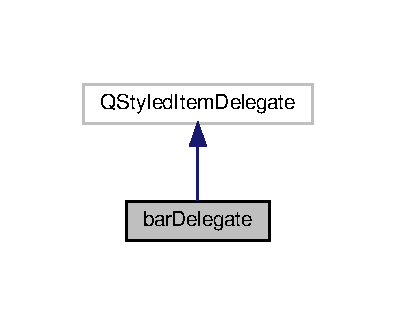
\includegraphics[width=190pt]{classbar_delegate__inherit__graph}
\end{center}
\end{figure}


Collaboration diagram for bar\+Delegate\+:\nopagebreak
\begin{figure}[H]
\begin{center}
\leavevmode
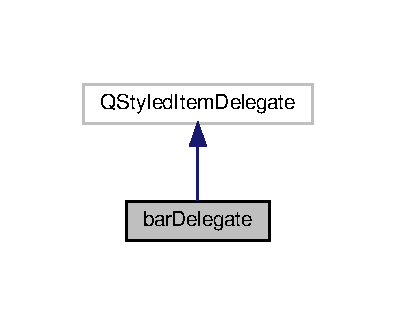
\includegraphics[width=190pt]{classbar_delegate__coll__graph}
\end{center}
\end{figure}
\subsection*{Public Member Functions}
\begin{DoxyCompactItemize}
\item 
\mbox{\Hypertarget{classbar_delegate_af31b0c196427b7856e88167594253f44}\label{classbar_delegate_af31b0c196427b7856e88167594253f44}} 
{\bfseries bar\+Delegate} (Q\+Widget $\ast$parent=0)
\item 
\mbox{\Hypertarget{classbar_delegate_ab3f8bec486210494bdd9ecb7179ef355}\label{classbar_delegate_ab3f8bec486210494bdd9ecb7179ef355}} 
void {\bfseries paint} (Q\+Painter $\ast$painter, const Q\+Style\+Option\+View\+Item \&option, const Q\+Model\+Index \&index) const override
\end{DoxyCompactItemize}


The documentation for this class was generated from the following files\+:\begin{DoxyCompactItemize}
\item 
bar\+Delegate.\+h\item 
bar\+Delegate.\+cpp\end{DoxyCompactItemize}

\hypertarget{class_boolean_delegate}{}\section{Boolean\+Delegate Class Reference}
\label{class_boolean_delegate}\index{Boolean\+Delegate@{Boolean\+Delegate}}


Inheritance diagram for Boolean\+Delegate\+:\nopagebreak
\begin{figure}[H]
\begin{center}
\leavevmode
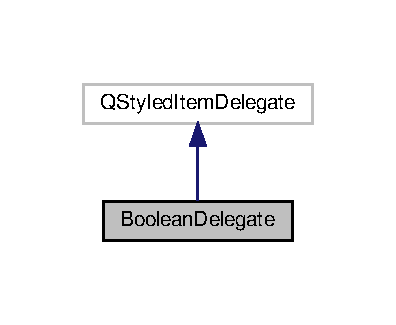
\includegraphics[width=190pt]{class_boolean_delegate__inherit__graph}
\end{center}
\end{figure}


Collaboration diagram for Boolean\+Delegate\+:\nopagebreak
\begin{figure}[H]
\begin{center}
\leavevmode
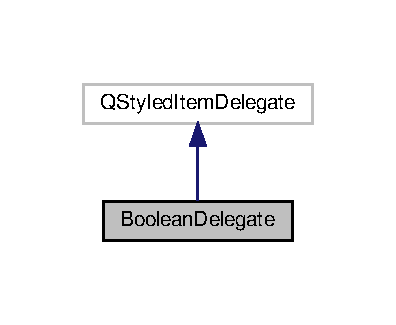
\includegraphics[width=190pt]{class_boolean_delegate__coll__graph}
\end{center}
\end{figure}
\subsection*{Public Member Functions}
\begin{DoxyCompactItemize}
\item 
\mbox{\Hypertarget{class_boolean_delegate_aacc5bab39e69a82f31f52881441abc08}\label{class_boolean_delegate_aacc5bab39e69a82f31f52881441abc08}} 
{\bfseries Boolean\+Delegate} (Q\+Object $\ast$parent=0)
\item 
\mbox{\Hypertarget{class_boolean_delegate_a75f9ded6d0eeefef5d1a5ca1f0f51b46}\label{class_boolean_delegate_a75f9ded6d0eeefef5d1a5ca1f0f51b46}} 
void {\bfseries paint} (Q\+Painter $\ast$painter, const Q\+Style\+Option\+View\+Item \&option, const Q\+Model\+Index \&index) const override
\item 
\mbox{\Hypertarget{class_boolean_delegate_a161b7bcc5d5b0ef3022fb0bec0d5de52}\label{class_boolean_delegate_a161b7bcc5d5b0ef3022fb0bec0d5de52}} 
bool {\bfseries editor\+Event} (Q\+Event $\ast$event, Q\+Abstract\+Item\+Model $\ast$model, const Q\+Style\+Option\+View\+Item \&option, const Q\+Model\+Index \&index)
\end{DoxyCompactItemize}


The documentation for this class was generated from the following files\+:\begin{DoxyCompactItemize}
\item 
booleaneditor.\+h\item 
booleaneditor.\+cpp\end{DoxyCompactItemize}

\hypertarget{classmz_file_loader}{}\section{mz\+File\+Loader Class Reference}
\label{classmz_file_loader}\index{mz\+File\+Loader@{mz\+File\+Loader}}


The \mbox{\hyperlink{classmz_file_loader}{mz\+File\+Loader}} class.  




{\ttfamily \#include $<$mzfileloader.\+h$>$}



Inheritance diagram for mz\+File\+Loader\+:\nopagebreak
\begin{figure}[H]
\begin{center}
\leavevmode
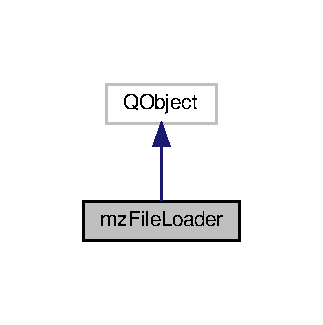
\includegraphics[width=155pt]{classmz_file_loader__inherit__graph}
\end{center}
\end{figure}


Collaboration diagram for mz\+File\+Loader\+:\nopagebreak
\begin{figure}[H]
\begin{center}
\leavevmode
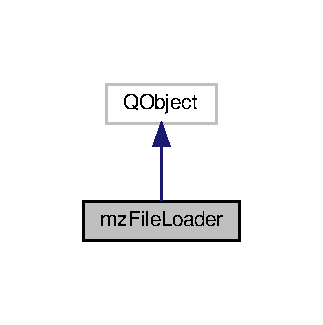
\includegraphics[width=155pt]{classmz_file_loader__coll__graph}
\end{center}
\end{figure}
\subsection*{Public Slots}
\begin{DoxyCompactItemize}
\item 
\mbox{\Hypertarget{classmz_file_loader_acddd84704393e54d2e3c48e999a55b15}\label{classmz_file_loader_acddd84704393e54d2e3c48e999a55b15}} 
void \mbox{\hyperlink{classmz_file_loader_acddd84704393e54d2e3c48e999a55b15}{load}} ()
\begin{DoxyCompactList}\small\item\em This slot is connected to the \char`\"{}\+Load File...\char`\"{}-\/button. This gets everything going. Opens a file dialog to select file to load, then invokes the parser to attempt to parse it. If successful, fills protein and peptide tables with read data. \end{DoxyCompactList}\end{DoxyCompactItemize}
\subsection*{Signals}
\begin{DoxyCompactItemize}
\item 
\mbox{\Hypertarget{classmz_file_loader_ad2b2290c7dcf0859f02fd43bc75491a6}\label{classmz_file_loader_ad2b2290c7dcf0859f02fd43bc75491a6}} 
void \mbox{\hyperlink{classmz_file_loader_ad2b2290c7dcf0859f02fd43bc75491a6}{clear\+Combo\+Box}} ()
\begin{DoxyCompactList}\small\item\em This signal is used to clear the combobox(es) of all entries when loading new files. \end{DoxyCompactList}\item 
void \mbox{\hyperlink{classmz_file_loader_ae659f02714e23607b981617155302f71}{Header\+Data\+Changed}} (Q\+String\+List headers)
\begin{DoxyCompactList}\small\item\em This signal is used to insert new selectable items into the search combobox(es) when loading new files. \end{DoxyCompactList}\end{DoxyCompactItemize}
\subsection*{Public Member Functions}
\begin{DoxyCompactItemize}
\item 
void \mbox{\hyperlink{classmz_file_loader_a699254cd8dabbf7fda70f02aa06730f7}{set\+Models}} (Q\+Standard\+Item\+Model $\ast$first\+Model, Q\+Standard\+Item\+Model $\ast$second\+Model)
\begin{DoxyCompactList}\small\item\em This function makes both base models available in this class. \end{DoxyCompactList}\item 
void \mbox{\hyperlink{classmz_file_loader_a515cf8ce62e8c7c235a62536e739cb9d}{set\+Proxies}} (Q\+Sort\+Filter\+Proxy\+Model $\ast$first\+Proxy, Q\+Sort\+Filter\+Proxy\+Model $\ast$second\+Proxy, Q\+Sort\+Filter\+Proxy\+Model $\ast$third\+Proxy, Q\+Sort\+Filter\+Proxy\+Model $\ast$fourth\+Proxy, Q\+Sort\+Filter\+Proxy\+Model $\ast$pep\+Proxy)
\begin{DoxyCompactList}\small\item\em This function makes all proxies available in this class. \end{DoxyCompactList}\item 
void \mbox{\hyperlink{classmz_file_loader_a92066953ae94c2cf1e58a2bf4a95c021}{set\+Table\+Views}} (Q\+Table\+View $\ast$first\+Table, Q\+Table\+View $\ast$second\+Table)
\begin{DoxyCompactList}\small\item\em This function makes both Table\+Views available in this class. \end{DoxyCompactList}\item 
\mbox{\hyperlink{structmz_tab_file}{mz\+Tab\+File}} \mbox{\hyperlink{classmz_file_loader_a495d5ddac38877451d24d974c25f7f11}{get\+Data}} ()
\begin{DoxyCompactList}\small\item\em This function is currently unused. It returns the remaining structure left over after inserting into the model. Maybe someday someone has to look at the leftovers... \end{DoxyCompactList}\end{DoxyCompactItemize}


\subsection{Detailed Description}
The \mbox{\hyperlink{classmz_file_loader}{mz\+File\+Loader}} class. 

Loader that opens file select dialogue, activates parser and fills models. This class acts as a controller and has access to all important objects to be able to efficiently load data. 

\subsection{Member Function Documentation}
\mbox{\Hypertarget{classmz_file_loader_a495d5ddac38877451d24d974c25f7f11}\label{classmz_file_loader_a495d5ddac38877451d24d974c25f7f11}} 
\index{mz\+File\+Loader@{mz\+File\+Loader}!get\+Data@{get\+Data}}
\index{get\+Data@{get\+Data}!mz\+File\+Loader@{mz\+File\+Loader}}
\subsubsection{\texorpdfstring{get\+Data()}{getData()}}
{\footnotesize\ttfamily \mbox{\hyperlink{structmz_tab_file}{mz\+Tab\+File}} mz\+File\+Loader\+::get\+Data (\begin{DoxyParamCaption}{ }\end{DoxyParamCaption})\hspace{0.3cm}{\ttfamily [inline]}}



This function is currently unused. It returns the remaining structure left over after inserting into the model. Maybe someday someone has to look at the leftovers... 

\begin{DoxyReturn}{Returns}
An \mbox{\hyperlink{structmz_tab_file}{mz\+Tab\+File}} structure (may be empty or only contain metadata) 
\end{DoxyReturn}
\mbox{\Hypertarget{classmz_file_loader_ae659f02714e23607b981617155302f71}\label{classmz_file_loader_ae659f02714e23607b981617155302f71}} 
\index{mz\+File\+Loader@{mz\+File\+Loader}!Header\+Data\+Changed@{Header\+Data\+Changed}}
\index{Header\+Data\+Changed@{Header\+Data\+Changed}!mz\+File\+Loader@{mz\+File\+Loader}}
\subsubsection{\texorpdfstring{Header\+Data\+Changed}{HeaderDataChanged}}
{\footnotesize\ttfamily void mz\+File\+Loader\+::\+Header\+Data\+Changed (\begin{DoxyParamCaption}\item[{Q\+String\+List}]{headers }\end{DoxyParamCaption})\hspace{0.3cm}{\ttfamily [signal]}}



This signal is used to insert new selectable items into the search combobox(es) when loading new files. 


\begin{DoxyParams}{Parameters}
{\em headers} & The selectable headers \\
\hline
\end{DoxyParams}
\mbox{\Hypertarget{classmz_file_loader_a699254cd8dabbf7fda70f02aa06730f7}\label{classmz_file_loader_a699254cd8dabbf7fda70f02aa06730f7}} 
\index{mz\+File\+Loader@{mz\+File\+Loader}!set\+Models@{set\+Models}}
\index{set\+Models@{set\+Models}!mz\+File\+Loader@{mz\+File\+Loader}}
\subsubsection{\texorpdfstring{set\+Models()}{setModels()}}
{\footnotesize\ttfamily void mz\+File\+Loader\+::set\+Models (\begin{DoxyParamCaption}\item[{Q\+Standard\+Item\+Model $\ast$}]{first\+Model,  }\item[{Q\+Standard\+Item\+Model $\ast$}]{second\+Model }\end{DoxyParamCaption})\hspace{0.3cm}{\ttfamily [inline]}}



This function makes both base models available in this class. 


\begin{DoxyParams}{Parameters}
{\em first\+Model} & The protein base model \\
\hline
{\em second\+Model} & The peptide base model \\
\hline
\end{DoxyParams}
\mbox{\Hypertarget{classmz_file_loader_a515cf8ce62e8c7c235a62536e739cb9d}\label{classmz_file_loader_a515cf8ce62e8c7c235a62536e739cb9d}} 
\index{mz\+File\+Loader@{mz\+File\+Loader}!set\+Proxies@{set\+Proxies}}
\index{set\+Proxies@{set\+Proxies}!mz\+File\+Loader@{mz\+File\+Loader}}
\subsubsection{\texorpdfstring{set\+Proxies()}{setProxies()}}
{\footnotesize\ttfamily void mz\+File\+Loader\+::set\+Proxies (\begin{DoxyParamCaption}\item[{Q\+Sort\+Filter\+Proxy\+Model $\ast$}]{first\+Proxy,  }\item[{Q\+Sort\+Filter\+Proxy\+Model $\ast$}]{second\+Proxy,  }\item[{Q\+Sort\+Filter\+Proxy\+Model $\ast$}]{third\+Proxy,  }\item[{Q\+Sort\+Filter\+Proxy\+Model $\ast$}]{fourth\+Proxy,  }\item[{Q\+Sort\+Filter\+Proxy\+Model $\ast$}]{pep\+Proxy }\end{DoxyParamCaption})\hspace{0.3cm}{\ttfamily [inline]}}



This function makes all proxies available in this class. 


\begin{DoxyParams}{Parameters}
{\em first\+Proxy} & The protein proxy model lowest in the stack \\
\hline
{\em second\+Proxy} & The protein proxy model second lowest in the stack \\
\hline
{\em third\+Proxy} & The protein proxy model second highest in the stack \\
\hline
{\em fourth\+Proxy} & The protein proxy model highest in the stack \\
\hline
{\em pep\+Proxy} & The peptide proxy model (it only needs one) \\
\hline
\end{DoxyParams}
\mbox{\Hypertarget{classmz_file_loader_a92066953ae94c2cf1e58a2bf4a95c021}\label{classmz_file_loader_a92066953ae94c2cf1e58a2bf4a95c021}} 
\index{mz\+File\+Loader@{mz\+File\+Loader}!set\+Table\+Views@{set\+Table\+Views}}
\index{set\+Table\+Views@{set\+Table\+Views}!mz\+File\+Loader@{mz\+File\+Loader}}
\subsubsection{\texorpdfstring{set\+Table\+Views()}{setTableViews()}}
{\footnotesize\ttfamily void mz\+File\+Loader\+::set\+Table\+Views (\begin{DoxyParamCaption}\item[{Q\+Table\+View $\ast$}]{first\+Table,  }\item[{Q\+Table\+View $\ast$}]{second\+Table }\end{DoxyParamCaption})\hspace{0.3cm}{\ttfamily [inline]}}



This function makes both Table\+Views available in this class. 


\begin{DoxyParams}{Parameters}
{\em first\+Table} & The protein table \\
\hline
{\em second\+Table} & The peptide table \\
\hline
\end{DoxyParams}


The documentation for this class was generated from the following files\+:\begin{DoxyCompactItemize}
\item 
mzfileloader.\+h\item 
mzfileloader.\+cpp\end{DoxyCompactItemize}

\hypertarget{classmz_parser}{}\section{mz\+Parser Class Reference}
\label{classmz_parser}\index{mz\+Parser@{mz\+Parser}}


The \mbox{\hyperlink{classmz_parser}{mz\+Parser}} class.  




{\ttfamily \#include $<$mzparser.\+h$>$}

\subsection*{Public Member Functions}
\begin{DoxyCompactItemize}
\item 
\mbox{\hyperlink{structmz_tab_file}{mz\+Tab\+File}} \mbox{\hyperlink{classmz_parser_aaff07e834a579526b82e86a7bd026d1f}{parse}} (std\+::string path)
\begin{DoxyCompactList}\small\item\em This function encompasses everything this class does. Open a file at given path and read data. Fill \mbox{\hyperlink{structmz_tab_file}{mz\+Tab\+File}} structure with data. Hand structure off to be handled by the loader. \end{DoxyCompactList}\end{DoxyCompactItemize}
\subsection*{Static Public Member Functions}
\begin{DoxyCompactItemize}
\item 
static \mbox{\hyperlink{classmz_parser}{mz\+Parser}} \& \mbox{\hyperlink{classmz_parser_a8838850b084cdc867b2b03122de5401b}{instance}} ()
\begin{DoxyCompactList}\small\item\em This function returns the single instance of the parser. \end{DoxyCompactList}\end{DoxyCompactItemize}


\subsection{Detailed Description}
The \mbox{\hyperlink{classmz_parser}{mz\+Parser}} class. 

Singleton parser for files in mz\+Tab format. Opens file at given path and tries to fill an \mbox{\hyperlink{structmz_tab_file}{mz\+Tab\+File}} structure with the data read. 

\subsection{Member Function Documentation}
\mbox{\Hypertarget{classmz_parser_a8838850b084cdc867b2b03122de5401b}\label{classmz_parser_a8838850b084cdc867b2b03122de5401b}} 
\index{mz\+Parser@{mz\+Parser}!instance@{instance}}
\index{instance@{instance}!mz\+Parser@{mz\+Parser}}
\subsubsection{\texorpdfstring{instance()}{instance()}}
{\footnotesize\ttfamily static \mbox{\hyperlink{classmz_parser}{mz\+Parser}}\& mz\+Parser\+::instance (\begin{DoxyParamCaption}{ }\end{DoxyParamCaption})\hspace{0.3cm}{\ttfamily [inline]}, {\ttfamily [static]}}



This function returns the single instance of the parser. 

\begin{DoxyReturn}{Returns}
The one and only instance 
\end{DoxyReturn}
\mbox{\Hypertarget{classmz_parser_aaff07e834a579526b82e86a7bd026d1f}\label{classmz_parser_aaff07e834a579526b82e86a7bd026d1f}} 
\index{mz\+Parser@{mz\+Parser}!parse@{parse}}
\index{parse@{parse}!mz\+Parser@{mz\+Parser}}
\subsubsection{\texorpdfstring{parse()}{parse()}}
{\footnotesize\ttfamily \mbox{\hyperlink{structmz_tab_file}{mz\+Tab\+File}} mz\+Parser\+::parse (\begin{DoxyParamCaption}\item[{std\+::string}]{path }\end{DoxyParamCaption})}



This function encompasses everything this class does. Open a file at given path and read data. Fill \mbox{\hyperlink{structmz_tab_file}{mz\+Tab\+File}} structure with data. Hand structure off to be handled by the loader. 


\begin{DoxyParams}{Parameters}
{\em path} & The path to the file to be read \\
\hline
\end{DoxyParams}
\begin{DoxyReturn}{Returns}
An \mbox{\hyperlink{structmz_tab_file}{mz\+Tab\+File}} structure. mz\+Tab\+File.\+is\+Valid == false in case of error 
\end{DoxyReturn}


The documentation for this class was generated from the following files\+:\begin{DoxyCompactItemize}
\item 
mzparser.\+h\item 
mzparser.\+cpp\end{DoxyCompactItemize}

\hypertarget{structmz_tab_file}{}\section{mz\+Tab\+File Struct Reference}
\label{structmz_tab_file}\index{mz\+Tab\+File@{mz\+Tab\+File}}


The \mbox{\hyperlink{structmz_tab_file}{mz\+Tab\+File}} struct.  




{\ttfamily \#include $<$mz\+Tab\+File.\+h$>$}

\subsection*{Public Attributes}
\begin{DoxyCompactItemize}
\item 
\mbox{\Hypertarget{structmz_tab_file_a6c20ef1e57959be37a12a6c77412ab50}\label{structmz_tab_file_a6c20ef1e57959be37a12a6c77412ab50}} 
std\+::map$<$ Q\+String, Q\+String $>$ {\bfseries metadata}
\item 
\mbox{\Hypertarget{structmz_tab_file_ad9b778603a2ea9c13dda56969c5a1c36}\label{structmz_tab_file_ad9b778603a2ea9c13dda56969c5a1c36}} 
Q\+List$<$ Q\+String\+List $>$ {\bfseries proteins}
\item 
\mbox{\Hypertarget{structmz_tab_file_a165994178856f810865df12b475a55a6}\label{structmz_tab_file_a165994178856f810865df12b475a55a6}} 
Q\+List$<$ Q\+String\+List $>$ {\bfseries peptides}
\item 
\mbox{\Hypertarget{structmz_tab_file_a72f3db89bd7aea763d4684b0f12247b6}\label{structmz_tab_file_a72f3db89bd7aea763d4684b0f12247b6}} 
Q\+List$<$ Q\+String\+List $>$ {\bfseries psm}
\item 
\mbox{\Hypertarget{structmz_tab_file_a66c3e1a512b70b9a8669b227c04846b0}\label{structmz_tab_file_a66c3e1a512b70b9a8669b227c04846b0}} 
Q\+List$<$ Q\+String\+List $>$ {\bfseries small\+Molecules}
\item 
\mbox{\Hypertarget{structmz_tab_file_a5724e0be23c7762c23e4ffce0d297588}\label{structmz_tab_file_a5724e0be23c7762c23e4ffce0d297588}} 
bool {\bfseries is\+Valid} = true
\end{DoxyCompactItemize}


\subsection{Detailed Description}
The \mbox{\hyperlink{structmz_tab_file}{mz\+Tab\+File}} struct. 

Struct to contain data read from file and save it in a way that\textquotesingle{}s relatively easy to access. is\+Valid denotes wether or not an error occurred during parsing. 

The documentation for this struct was generated from the following file\+:\begin{DoxyCompactItemize}
\item 
mz\+Tab\+File.\+h\end{DoxyCompactItemize}

\hypertarget{class_peptide_view}{}\section{Peptide\+View Class Reference}
\label{class_peptide_view}\index{Peptide\+View@{Peptide\+View}}


The \mbox{\hyperlink{class_peptide_view}{Peptide\+View}} class.  




{\ttfamily \#include $<$peptideview.\+h$>$}



Inheritance diagram for Peptide\+View\+:\nopagebreak
\begin{figure}[H]
\begin{center}
\leavevmode
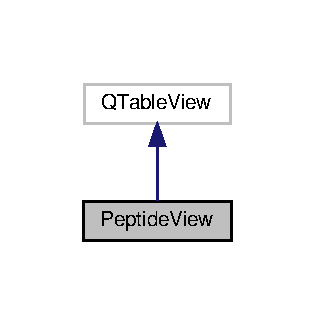
\includegraphics[width=151pt]{class_peptide_view__inherit__graph}
\end{center}
\end{figure}


Collaboration diagram for Peptide\+View\+:\nopagebreak
\begin{figure}[H]
\begin{center}
\leavevmode
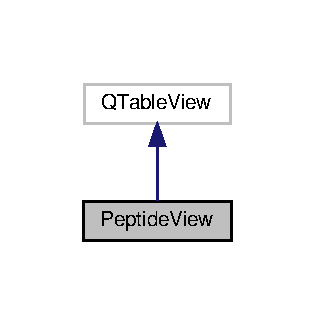
\includegraphics[width=151pt]{class_peptide_view__coll__graph}
\end{center}
\end{figure}
\subsection*{Public Slots}
\begin{DoxyCompactItemize}
\item 
void \mbox{\hyperlink{class_peptide_view_a44ff37ec18e1e1c61c8747b6fe79e076}{to\+Be\+Displayed}} (Q\+List$<$ Q\+String $>$)
\begin{DoxyCompactList}\small\item\em This function hides and shows rows according to its input. \end{DoxyCompactList}\item 
void \mbox{\hyperlink{class_peptide_view_ab96162d2cb5e04591e6225505afceefe}{update\+Event\+Star}} ()
\begin{DoxyCompactList}\small\item\em This function marks Stars. \end{DoxyCompactList}\item 
void \mbox{\hyperlink{class_peptide_view_a8f1b5cfad280a3eb8e4a290cdef588bd}{clear\+Selection}} ()
\begin{DoxyCompactList}\small\item\em The clear\+Selection function sets all items as unselected. \end{DoxyCompactList}\item 
\mbox{\Hypertarget{class_peptide_view_ab2e4b1c394cd47afec35baceedf8be07}\label{class_peptide_view_ab2e4b1c394cd47afec35baceedf8be07}} 
void \mbox{\hyperlink{class_peptide_view_ab2e4b1c394cd47afec35baceedf8be07}{clear\+Pep\+Star}} ()
\begin{DoxyCompactList}\small\item\em Clears all stars in the Peptide Table. \end{DoxyCompactList}\end{DoxyCompactItemize}
\subsection*{Signals}
\begin{DoxyCompactItemize}
\item 
\mbox{\Hypertarget{class_peptide_view_acaeeae28c65e40998f8b9f5eaf829f71}\label{class_peptide_view_acaeeae28c65e40998f8b9f5eaf829f71}} 
void \mbox{\hyperlink{class_peptide_view_acaeeae28c65e40998f8b9f5eaf829f71}{update\+Star}} ()
\begin{DoxyCompactList}\small\item\em This signal is a parameter free notification. \end{DoxyCompactList}\end{DoxyCompactItemize}
\subsection*{Protected Member Functions}
\begin{DoxyCompactItemize}
\item 
\mbox{\Hypertarget{class_peptide_view_a6c451e673bc3e13c3dfe1de10505f567}\label{class_peptide_view_a6c451e673bc3e13c3dfe1de10505f567}} 
bool {\bfseries event\+Filter} (Q\+Object $\ast$, Q\+Event $\ast$) override
\end{DoxyCompactItemize}


\subsection{Detailed Description}
The \mbox{\hyperlink{class_peptide_view}{Peptide\+View}} class. 

The \mbox{\hyperlink{class_peptide_view}{Peptide\+View}} class offers a customized version of the Q\+Table\+View class. In addition to the Q\+Table\+View functions it offers a slot which can hide and show rows depending on given entries. 

\subsection{Member Function Documentation}
\mbox{\Hypertarget{class_peptide_view_a8f1b5cfad280a3eb8e4a290cdef588bd}\label{class_peptide_view_a8f1b5cfad280a3eb8e4a290cdef588bd}} 
\index{Peptide\+View@{Peptide\+View}!clear\+Selection@{clear\+Selection}}
\index{clear\+Selection@{clear\+Selection}!Peptide\+View@{Peptide\+View}}
\subsubsection{\texorpdfstring{clear\+Selection}{clearSelection}}
{\footnotesize\ttfamily void Peptide\+View\+::clear\+Selection (\begin{DoxyParamCaption}{ }\end{DoxyParamCaption})\hspace{0.3cm}{\ttfamily [slot]}}



The clear\+Selection function sets all items as unselected. 

The function deselects all selected items and emits the \mbox{\hyperlink{class_peptide_view_acaeeae28c65e40998f8b9f5eaf829f71}{update\+Star()}} signal, indicating that the selection may have changed. \mbox{\Hypertarget{class_peptide_view_a44ff37ec18e1e1c61c8747b6fe79e076}\label{class_peptide_view_a44ff37ec18e1e1c61c8747b6fe79e076}} 
\index{Peptide\+View@{Peptide\+View}!to\+Be\+Displayed@{to\+Be\+Displayed}}
\index{to\+Be\+Displayed@{to\+Be\+Displayed}!Peptide\+View@{Peptide\+View}}
\subsubsection{\texorpdfstring{to\+Be\+Displayed}{toBeDisplayed}}
{\footnotesize\ttfamily void Peptide\+View\+::to\+Be\+Displayed (\begin{DoxyParamCaption}\item[{Q\+List$<$ Q\+String $>$}]{display\+These }\end{DoxyParamCaption})\hspace{0.3cm}{\ttfamily [slot]}}



This function hides and shows rows according to its input. 

to\+Be\+Displayed receives a List of accesion codes as Q\+Strings. If the model contains a column with header \char`\"{}accession\char`\"{} the function will set all rows as shown, for which the entries in the accession column are contained in the input, and set all columns as hidden for which the entries aren\textquotesingle{}t. If the model does not contain such a column, the function will return without doing anything. This function can be connected as a Slot


\begin{DoxyParams}{Parameters}
{\em Q\+List$<$\+Q\+String$>$} & contains a List of accession codes as Q\+Strings \\
\hline
\end{DoxyParams}
\mbox{\Hypertarget{class_peptide_view_ab96162d2cb5e04591e6225505afceefe}\label{class_peptide_view_ab96162d2cb5e04591e6225505afceefe}} 
\index{Peptide\+View@{Peptide\+View}!update\+Event\+Star@{update\+Event\+Star}}
\index{update\+Event\+Star@{update\+Event\+Star}!Peptide\+View@{Peptide\+View}}
\subsubsection{\texorpdfstring{update\+Event\+Star}{updateEventStar}}
{\footnotesize\ttfamily void Peptide\+View\+::update\+Event\+Star (\begin{DoxyParamCaption}{ }\end{DoxyParamCaption})\hspace{0.3cm}{\ttfamily [slot]}}



This function marks Stars. 

update\+Event\+Star unmarks all stars, checks which rows in the peptide table are selected and then marks stars in selected rows. 

The documentation for this class was generated from the following files\+:\begin{DoxyCompactItemize}
\item 
peptideview.\+h\item 
peptideview.\+cpp\end{DoxyCompactItemize}

\hypertarget{class_protein_view}{}\section{Protein\+View Class Reference}
\label{class_protein_view}\index{Protein\+View@{Protein\+View}}


Inheritance diagram for Protein\+View\+:\nopagebreak
\begin{figure}[H]
\begin{center}
\leavevmode
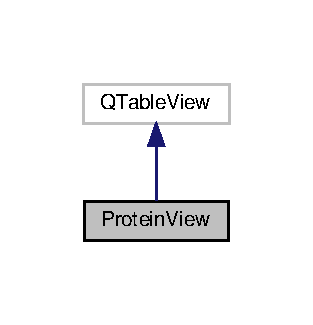
\includegraphics[width=150pt]{class_protein_view__inherit__graph}
\end{center}
\end{figure}


Collaboration diagram for Protein\+View\+:\nopagebreak
\begin{figure}[H]
\begin{center}
\leavevmode
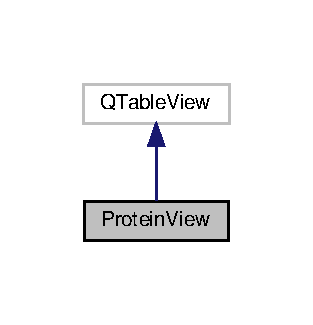
\includegraphics[width=150pt]{class_protein_view__coll__graph}
\end{center}
\end{figure}
\subsection*{Public Slots}
\begin{DoxyCompactItemize}
\item 
\mbox{\Hypertarget{class_protein_view_af352ac170651ea7d1ed401200a14c2c8}\label{class_protein_view_af352ac170651ea7d1ed401200a14c2c8}} 
void {\bfseries update\+Event} ()
\end{DoxyCompactItemize}
\subsection*{Signals}
\begin{DoxyCompactItemize}
\item 
\mbox{\Hypertarget{class_protein_view_a3293f5d199157bce7e98ea78171635c5}\label{class_protein_view_a3293f5d199157bce7e98ea78171635c5}} 
void {\bfseries released} ()
\item 
\mbox{\Hypertarget{class_protein_view_aea998af0dc44d2636dab2f8bdba07a66}\label{class_protein_view_aea998af0dc44d2636dab2f8bdba07a66}} 
void {\bfseries active\+Accessions} (Q\+List$<$ Q\+String $>$)
\end{DoxyCompactItemize}
\subsection*{Protected Member Functions}
\begin{DoxyCompactItemize}
\item 
\mbox{\Hypertarget{class_protein_view_ad6a88c7d11cfd0fef51f5e3da4cf3476}\label{class_protein_view_ad6a88c7d11cfd0fef51f5e3da4cf3476}} 
bool {\bfseries event\+Filter} (Q\+Object $\ast$, Q\+Event $\ast$) override
\end{DoxyCompactItemize}


The documentation for this class was generated from the following files\+:\begin{DoxyCompactItemize}
\item 
proteinview.\+h\item 
proteinview.\+cpp\end{DoxyCompactItemize}

\hypertarget{class_q_custom_sort_filter_proxy_model}{}\section{Q\+Custom\+Sort\+Filter\+Proxy\+Model Class Reference}
\label{class_q_custom_sort_filter_proxy_model}\index{Q\+Custom\+Sort\+Filter\+Proxy\+Model@{Q\+Custom\+Sort\+Filter\+Proxy\+Model}}


Inheritance diagram for Q\+Custom\+Sort\+Filter\+Proxy\+Model\+:\nopagebreak
\begin{figure}[H]
\begin{center}
\leavevmode
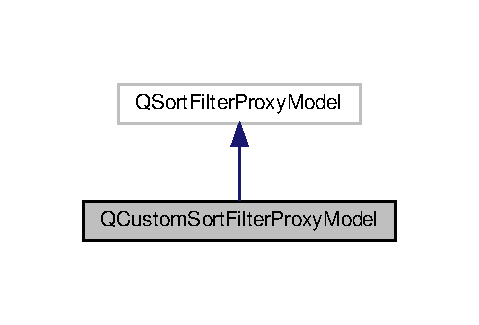
\includegraphics[width=230pt]{class_q_custom_sort_filter_proxy_model__inherit__graph}
\end{center}
\end{figure}


Collaboration diagram for Q\+Custom\+Sort\+Filter\+Proxy\+Model\+:\nopagebreak
\begin{figure}[H]
\begin{center}
\leavevmode
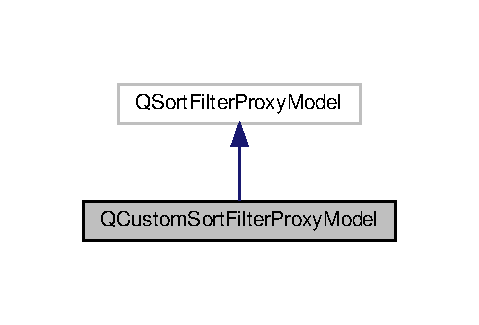
\includegraphics[width=230pt]{class_q_custom_sort_filter_proxy_model__coll__graph}
\end{center}
\end{figure}
\subsection*{Public Slots}
\begin{DoxyCompactItemize}
\item 
\mbox{\Hypertarget{class_q_custom_sort_filter_proxy_model_a32c931f0e638bb0f34090fd6beb622c8}\label{class_q_custom_sort_filter_proxy_model_a32c931f0e638bb0f34090fd6beb622c8}} 
void {\bfseries change\+Filter\+Key\+Column} (int col)
\item 
\mbox{\Hypertarget{class_q_custom_sort_filter_proxy_model_ace5bb8380d35be434b27a12afb10fd95}\label{class_q_custom_sort_filter_proxy_model_ace5bb8380d35be434b27a12afb10fd95}} 
void {\bfseries custom\+Set\+Filter\+Fixed\+String} (Q\+String)
\end{DoxyCompactItemize}
\subsection*{Signals}
\begin{DoxyCompactItemize}
\item 
\mbox{\Hypertarget{class_q_custom_sort_filter_proxy_model_a5032cbe24943fa9956d35148a65d0c89}\label{class_q_custom_sort_filter_proxy_model_a5032cbe24943fa9956d35148a65d0c89}} 
void {\bfseries model\+Updated} ()
\item 
\mbox{\Hypertarget{class_q_custom_sort_filter_proxy_model_a2449bf876853e7dcfc22a224873a8822}\label{class_q_custom_sort_filter_proxy_model_a2449bf876853e7dcfc22a224873a8822}} 
void {\bfseries update\+Filter} (Q\+String)
\end{DoxyCompactItemize}
\subsection*{Public Member Functions}
\begin{DoxyCompactItemize}
\item 
\mbox{\Hypertarget{class_q_custom_sort_filter_proxy_model_aa51b6a64ce00d57682fa21baa5c62f9e}\label{class_q_custom_sort_filter_proxy_model_aa51b6a64ce00d57682fa21baa5c62f9e}} 
{\bfseries Q\+Custom\+Sort\+Filter\+Proxy\+Model} (Q\+Object $\ast$parent=0)
\end{DoxyCompactItemize}


The documentation for this class was generated from the following files\+:\begin{DoxyCompactItemize}
\item 
qcustomsortfilterproxymodel.\+h\item 
qcustomsortfilterproxymodel.\+cpp\end{DoxyCompactItemize}

\hypertarget{classstar_delegate}{}\section{star\+Delegate Class Reference}
\label{classstar_delegate}\index{star\+Delegate@{star\+Delegate}}


Inheritance diagram for star\+Delegate\+:\nopagebreak
\begin{figure}[H]
\begin{center}
\leavevmode
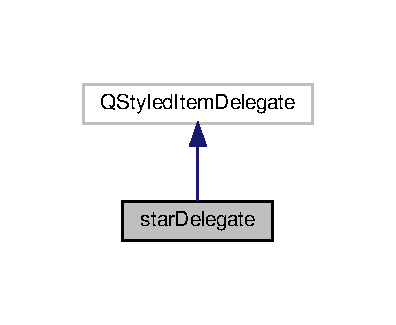
\includegraphics[width=190pt]{classstar_delegate__inherit__graph}
\end{center}
\end{figure}


Collaboration diagram for star\+Delegate\+:\nopagebreak
\begin{figure}[H]
\begin{center}
\leavevmode
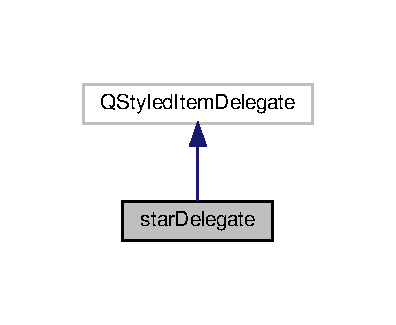
\includegraphics[width=190pt]{classstar_delegate__coll__graph}
\end{center}
\end{figure}
\subsection*{Public Member Functions}
\begin{DoxyCompactItemize}
\item 
\mbox{\Hypertarget{classstar_delegate_abf63fe9c7fe7e4c2253168e69eca595c}\label{classstar_delegate_abf63fe9c7fe7e4c2253168e69eca595c}} 
{\bfseries star\+Delegate} (Q\+Object $\ast$parent=0)
\item 
\mbox{\Hypertarget{classstar_delegate_a563a1503f4f1bd5e5f2d8762b95167c7}\label{classstar_delegate_a563a1503f4f1bd5e5f2d8762b95167c7}} 
void {\bfseries paint} (Q\+Painter $\ast$painter, const Q\+Style\+Option\+View\+Item \&option, const Q\+Model\+Index \&index) const override
\end{DoxyCompactItemize}


The documentation for this class was generated from the following files\+:\begin{DoxyCompactItemize}
\item 
star.\+h\item 
star.\+cpp\end{DoxyCompactItemize}

%--- End generated contents ---

% Index
\backmatter
\newpage
\phantomsection
\clearemptydoublepage
\addcontentsline{toc}{chapter}{\indexname}
\printindex

\end{document}
